Nous avons utilisé Git dès le début du projet, sachant qu'en plus, c'est l'un des gestionnaires de code le plus performant son utilisation était évidente
Git nous a permis de travailler séparement sans soucis. La prise en main s'est faite assez facilement car nous connaissions déjà cet outil, cela nous a donc permis d'en faire une utilisation plus poussée pour en avoir une meilleure gestion (utilisation de branches, des issues, ...).
Nous avons installé un depôt sur le Git du Sif. Nous avons utilisé une branche Master, qui devait contenir uniquement du code compilable, et après, chaque fonctionnalité a été développé sur une branche différente.
Nous utilisons également Gitg, pour avoir une meilleure vue de l'état de notre dêpot (cf~\ref{Gitg}) .
\begin{figure}[h]
\caption{\label{Gitg} Capture de Gitg}
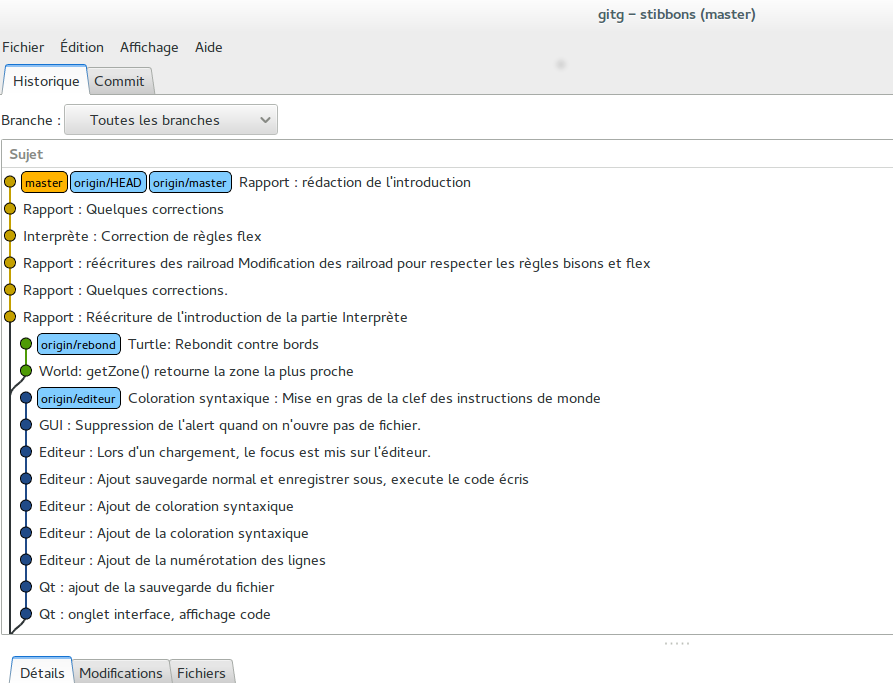
\includegraphics[scale=0.35]{doc/gestionProjet/gitbranche.png}
\end{figure}
% nb de ligne : wc -l `find . -name "*.h"` `find . -name "*.cpp"` `find . -name "*.y\+"` `find . -name "*.l\+"`
A la fin du projet, nous avons 495 commits, avec une moyenne de 4,4 commits par jours, 12 branches, 0 tags (nous avons utilisé les branches en guises de label de versions), et notre dossier fait 22.86MB.\\
Globalement, la gestion avec Git s'est bien passé, il y a eu quelques merges, mais rien d'irréparable. 
\begin{figure}[h]
\caption{\label{branche} Capture des branches sur Gitlab}
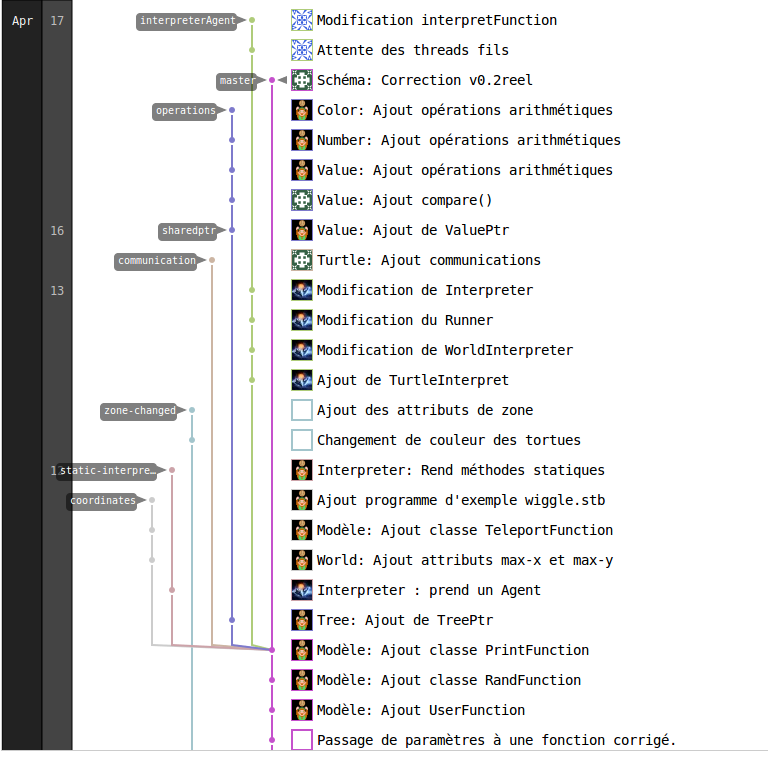
\includegraphics[scale=0.35]{doc/report/uml/network-v3.png}
\end{figure}
